%!TEX root = ../thesis.tex

\chapter{Scheduling}

\ifpdf
    \graphicspath{{Chapters/Figs/Raster/}{Chapters/Figs/PDF/}{Chapters/Figs/}}
\else
    \graphicspath{{Chapters/Figs/Vector/}{Chapters/Figs/}}
\fi

%********************************** % Intro *****************************************
In this chapter a scheduling framework for mixed-critical applications with precedence constraint and communication costs is presented.

%********************************** % Section  **************************************
\section{Introduction}
\par It has been shown \cite{MCSNPhard} that the mixed-criticality schedulability problem (preemptive or non-preemptive) is strongly NP-hard even with only two criticality levels (High and Low). Nevertheless, different approaches had been proposed in the literature. The first research was presented in 2009 by Anderson et al.\cite{Anderson09} and extended in 2010 \cite{Mollison10}. The mechanism they presented is based on assigning to high-critical tasks higher Worst Case Execution Time and different scheduling policies (e.g. level A tasks are statistic assigned and cyclic released, level B with a Partitioned-EDF scheduler, level C and D with G-EDF). Kritikakou et al.\cite{Kritikakou14} provided a new scheduling for tasks distinguished in only two levels: HI-criticality and LO-criticality. Same as proposed by S.Baruah et al.\cite{Baruah2012EDFVD} in which they describe EDF-VD (for Earliest Deadline First with Virtual Deadlines)  for mixed-criticality tasks (see \cite{Zhang2014} for detailed analysis).

%\paragraph{} In the following sections is presented a model to schedule real-time, mixed-critical task-sets with precedence and periodicity through an off-line scheduling algorithm.
\paragraph{}To properly treat the problem an formal abstraction of the real-time scheduling with mixed-critical tasks with precedence and periodicity is presented.

%********************************** % Section  **************************************
\section{Problem Formulation}
As stated in the previous chapter, tasks (or threads) to be scheduled are represented as an acyclic directed graph. Every node in the graph represents one task and the edges between nodes, the communications. The node cost is the time required for the task to complete (WCET) and the edge cost is the communication cost. 

\paragraph{} More formally, the tasks are defined by $G=(\Gamma,E,C,T,K)$ where $\tau_i\in\Gamma$ represents a task and $\Gamma$ the task-set. The set $E=\{e_{ij}:\forall\tau_i\to\tau_j\}$ represent the precedence constraints between $\tau_i$ and $\tau_j$ (meaning that $\tau_i$ must be completed before $\tau_j$) with its communication cost expressed in time. The Worst-Case Execution Times are expressed in $C=\{c_i:\forall\tau_i\in\Gamma\}$. The periods (or rate) are $T=\{T_i:\forall\tau_i\in\Gamma\}$ and it is assumed that every $T_i$ is a integer multiple of some base-period $\beta_T$. The criticality levels are $K=\{\chi:\forall\tau_i\in\Gamma\}$. Moreover, each task has its priority $\rho_i$ which is assigned by the scheduling algorithm and a set of accessed resources $\mathbb{R}$ manually assigned by the system designer to each task.
\par The Direct Acyclic Graph made by all the partitions (which are the group of tasks) is denoted by $\mathbb{P}=(\Pi, H, L, R)$ and called \emph{P-DAG}, where $\pi_i\in\Pi$ is a partition. The inter-partition communications are represented in $H$, $\lambda_i\in L$ and $\delta_i\in R$ are respectively the duration and the periodicity of the partition $\pi_i$. So we can define a map $\Psi:\Gamma\to\mathbb{P}$ as the partitioning algorithm. The subgraph of $G$ made by all the tasks assigned to a given partition is called T-DAG.
\par The behavioral parameters for the task $\tau_i$ that the scheduling process must define are: the starting time $s_i$ (\emph{when} the task should execute), and the core $\mu_i$ on which it will execute (\emph{where} should execute), also called \emph{affinity mask}.

%********************************** % Section  **************************************
\section{Assumptions}
It is assumed that the COTS board is a connected network of processors with identical communication links (the Unified Memory Model shown in figure \ref{fig:unifiedmemorymodel}) and relatively small number of processors. This simplifies the mathematical formulation of the optimization problem and limits its computational complexity.
\par It is also assumed that the partitioning addresses the security and safety requirement. This mechanism relies on the Hypervisor, which is a trusted code (certified by the authorities) and it is the only one executing in the highest privileged mode. It ensures time and spatial isolation among partitions so the partitioning algorithm should map each task to one partition such that a fault in one partition does not affect another partition while considering the criticality as a decision variable. Moreover, interferences and  inter-partition communications should be minimized.

\paragraph{} Once partitions are determined, they need to be scheduled. The problem can be split in two parts: \emph{intra-partition} scheduling and \emph{inter-partition} scheduling. In the following sections is presented a detailed description of each phase.

%********************************** % Section  **************************************
\section{Partitioning}
Determine a way to measure safety is complex, hence, derive an optimization problem is not easy. In order to simplify the intra-partition scheduling and enforce determinism it is important that all the tasks inside a partition have the same period (or eventually integer multiple of the partition rate). To understand the rationale, assume that a task $\tau_i$ assigned to \TP{1} needs to be activated at time $t_1<t_{L_1}$ and $t_2>t_{L_2}$ as shown in figure \ref{fig:PartitionRationale}
\begin{figure}[htbp] 
\centering    
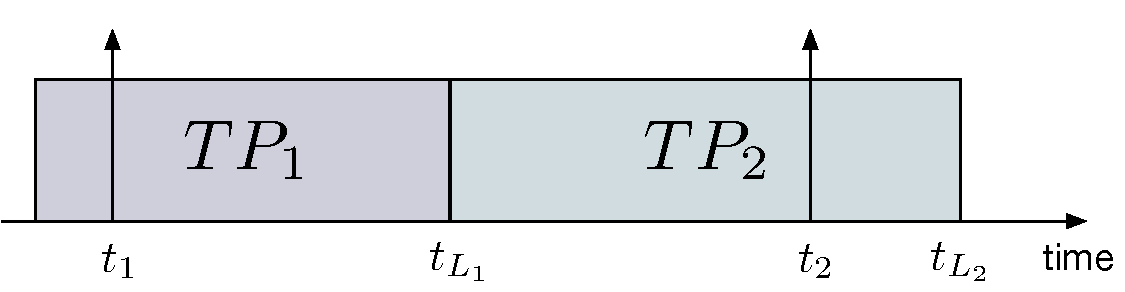
\includegraphics[width=0.7\textwidth]{PartitionRationale}
\caption{Non rate-base partitioning}
\label{fig:PartitionRationale}
\end{figure}

To allow this behavior, two approaches are possible:
\begin{enumerate}
\item Introduce preemption among time partition, losing determinism and the control of safety states.
\item Push the execution of $\tau_i$ o the new activation of \TP{1}. This approach leads to a lower level of determinism because $\tau_i$ now should interrupt any task assigned to \TP{2} that is executing at time $t_2$. Moreover, the worst-case execution time of \TP{2} will considerably change between different execution, leading to an over-estimating of it.
\end{enumerate}
The solution adopted in this work does not pretend to be a solution for the partitioning problem. Instead, it would be an example. The algorithm simply groups all the tasks with the same rates in partitions and then split them according to some criticality threshold, creating smaller sub-partitions. A more complex partitioning algorithm is under development.
\par As stated before, the result of the partitioning is another DAG, called P-DAG, each of them with its T-DAG. Now the inter-partition and intra-partition scheduling can be introduced. 

%********************************** % Section  **************************************
\section{Tasks Allocation and Scheduling}
\subsection{Intra-Partition}
In order to schedule partitions the execution time of the partition itself must be estimated. This optimization schedules a T-DAG on all the available $|M|$ processors. The solution space of this problem is spawned by all possible processor assignments combined with all possible task orderings that satisfy the partial order expressed by the T-DAG. The tasks are to be assigned in such a way as to minimize the total computation time required to execute that partition. This is also referred as reducing the makespan. The optimization problem that solves this problem presented below is based on the one proposed by S.Venugopalan and O.Sinnen \cite{ILP}.

\paragraph{} For each task $\tau_i\in\Gamma$, let $s_i$ the starting time, $\mu_i$ the core on which it will be executed and $\gamma_i$ the cost of all outgoing communications. Let $W$ the makespan and $|M|$ the number of available cores. Moreover, let $\delta^-(i)$ the set of tasks that need to be completed before task $\tau_i$. Some tasks cannot execute in parallel with another due the shared resource they are going to use, $\mathcal{I}$ is matrix that represent \emph{parallel incompatibilities}, the component $\mathcal{I}_{ij}$ is equal to one if $\tau_i$ and $\tau_j$ cannot execute in parallel, formally:
\[
\mathcal{I}_{i,j}=
\begin{cases}
1\quad \text{if } \tau_i \text{ and } \tau_j \text{ share at least one resource}\\
0\quad\text{otherwise}
\end{cases}
\]
Let the variable $x_{ik}$ is one if task $\tau_i$ is assigned to the processor $\mu_k$, zero otherwise. In order to control the scheduling behavior, define the following set of binary variables:
\[
\forall \tau_i,\tau_j\in\Gamma \quad \sigma_{ij}=
\begin{cases}
1\quad s_i+c_i\leq s_j \\
0\quad\text{otherwise}
\end{cases}
\]
\[
\forall \tau_i,\tau_j\in\Gamma \quad \epsilon_{ij}=
\begin{cases}
1\quad\mu_i<\mu_j \\
0\quad\text{otherwise}
\end{cases}
\]
The resulting MILP problem is
\begin{align}
\min    										& \quad & W \label{eq:milp1}\\
\forall\tau_i\in\Gamma							&  &  s_i+c_i\leq W \label{eq:milp2}\\
\forall\tau_i\neq\tau_j\in\Gamma				&  &  s_j-s_i-c_i-\gamma_i-(\sigma_{ij}-1)W_{\max}\geq 0 \label{eq:milp3}\\
\forall\tau_i\neq\tau_j\in\Gamma				&  &  \mu_j-\mu_i-1-(\epsilon_{ij}-1)M\geq 0 \label{eq:milp4}\\
\forall\tau_i\neq\tau_j\in\Gamma				&  &  \sigma_{ij}+\sigma_{ji}+\epsilon_{ij}+\epsilon_{ji}\geq 1 \label{eq:milp5}\\
\forall(i,j):\mathcal{I}_{ij}=1 				&  &  s_i+c_i+\gamma_i-s_j\leq W_{\max}(1-\sigma_{ij}) \label{eq:milp6}\\
\forall(i,j):\mathcal{I}_{ij}=1					&  &  s_j+c_j+\gamma_j-s_i\leq W_{\max}\sigma_{ij} \label{eq:milp7}\\
\forall\tau_i\neq\tau_j\in\Gamma				&  &  \sigma_{ij}+\sigma_{ji}\leq 1 \label{eq:milp8}\\
\forall\tau_i\neq\tau_j\in\Gamma				&  &  \epsilon_{ij}+\epsilon_{ji}\leq 1 \label{eq:milp9}\\
\forall\tau_j\in\Gamma:\tau_i\in\delta^-(j)		&  &  \sigma_{ij}=1 \label{eq:milp10}\\
\forall\tau_i\in\Gamma 							&  & \sum_{k\in |M|} kx_{ik}=\mu_i \label{eq:milp11}\\
\forall\tau_i\in\Gamma 							&  & \sum_{k\in |M|} x_{ik}=1 \label{eq:milp12}\\
												&  & 0\leq W \leq W_{\max} \label{eq:milp13}\\
\forall\tau_i\in\Gamma 							&  & s_i\geq 0 \label{eq:milp14}\\
\forall\tau_i\in\Gamma 							& & \mu_i\in \{1,...,|M|\} \label{eq:milp15}\\
\forall\tau_i\in\Gamma,k\in |M|					& & x_{ij}\in\{0,1\} \label{eq:milp16}\\
\forall\tau_i,\tau_j\in\Gamma					& & \sigma_{ij},\epsilon_{ij} \in\{0,1\} \label{eq:milp17}
\end{align}
Where $W_{\max}$ is an upper bound for the makespan $W$. It can be computed as all the tasks were executed on a single core (so it is the sum of computational cost and communication costs) or with some heuristics. 
\par The formulation is a min-max problem: this is achieved by minimizing the makespan $W$ while introducing the constraint (\ref{eq:milp2}). Constraint (\ref{eq:milp3}) impose the partial order on the tasks in terms of the $\sigma$ variables. Constraint (\ref{eq:milp4}) impose the multi-core usage. Constraint (\ref{eq:milp5}) impose that at least one of the following is true: $\tau_i$ must finish before $\tau_j$ starts and/or $\mu_i<\mu_j$. Constraints (\ref{eq:milp6}) and (\ref{eq:milp7}) avoid that two tasks that share a common resource execute in parallel. By (\ref{eq:milp8}) and (\ref{eq:milp9}) a task cannot be before and after another task in both time and cores. Constraint (\ref{eq:milp10}) enforces the task precedences defined by the T-DAG. Constraints (\ref{eq:milp11}) link the assignment variable $x$ with the core variables $\mu$ and finally (\ref{eq:milp12}) ensures that any given task runs only on one core.
\par The complexity in terms of constraint and variables, depends on $|G|$, $|E|$, $|M|$ and $|\mathcal{I}|$. Assuming that the number of processor $|M|$ and the number of shared resources $|\mathcal{I}|$ are small, then the MILP complexity is dominated by (\ref{eq:milp10}) which generates $O(|G||E|)$ constraints. In the worst case scenario $|E|=|G|(|G|-1)/2$, however, for task-sets representing real applications, we usually have $O(|E|)=O(|G|)$, hence the overall complexity is $O(|G|^2)$.

\paragraph{} Once a T-DAG related to a partition is scheduled the makespan of the schedule is the Worst-Case Execution Time of the partition itself. Moreover, the variables $s_i$ and $\mu_i$ for each task $\tau_i\in\Gamma$ are known so the priorities can be computed.

\subsection{Inter-Partition}\label{interpartition}
The inter-partition schedule is analogue to the problem of schedule the P-DAG on a single core. Indeed, each Resource Partition is assigned to a Time Partition that is as big the total Worst-Case-Execution-Time of the Resource Partition contained (this amount of time can be estimated after the intra-partition schedule). In PikeOS, Time partitions are scheduled according to a statically-assigned schedule scheme like they were on a single core.
\par The problem of scheduling tasks on a single core have received substantial attention and many algorithms are available in the literature, for a complete review see \cite{buttazzoRT} and \cite{blazewiczScheduling}.

\paragraph{} When scheduling the P-DAG, the partial order expressed by it must be satisfied. Let introduce some concept (as in \cite{blazewiczScheduling}). For seek of notation simplicity, let consider a partition like a task, so that the same notation as before can be used. In addition to the previous notation, let introduce the \emph{arrival time} of a partition $\pi_i$ as $r_i$ which represent the moment in time in which a partition can start its execution, and the \emph{due date} $\widetilde{d}_i$ as the moment in time in which the task must be completed. These parameters, together with the periodicity, represent the real-time requirement for a given partition.

\subsubsection{Factorization}
Considering all nodes in the P-DAG, it is common to find different periodicity. In the general problem formulation is assumed that the periodicity of each task is an integer multiple of a base-period $\beta_T$, so when they are grouped into a partition, the partition itself inherit the rate of the tasks it contains and the so does the property. If $T_i=k_i\beta_T$ , the \emph{Hyper-Period} or \emph{Major Time Frame} can be defined as
\begin{equation}
\Delta = \gcd(k_1,k_2,...)\beta_T\quad i=\{1,...,|\Pi|\}
\end{equation}
Inside the hyper-period some partitions $\pi_i$ should execute more than once, in general exactly $k_i$ times. In order to generalize this behavior, a \emph{factorized P-DAG} can be defined. Let denote it as $\widetilde{\mathbb{P}}=(\widetilde{\Pi},\widetilde{H},\widetilde{L},\widetilde{R})$, it is a \emph{finite repetitive precedence} of partition $\pi_i$ by exactly $k_i$ times, in a direct precedence relation. The factorization process is depicted in figure \ref{fig:Factorization}.

\begin{figure}[htbp] 
\centering    
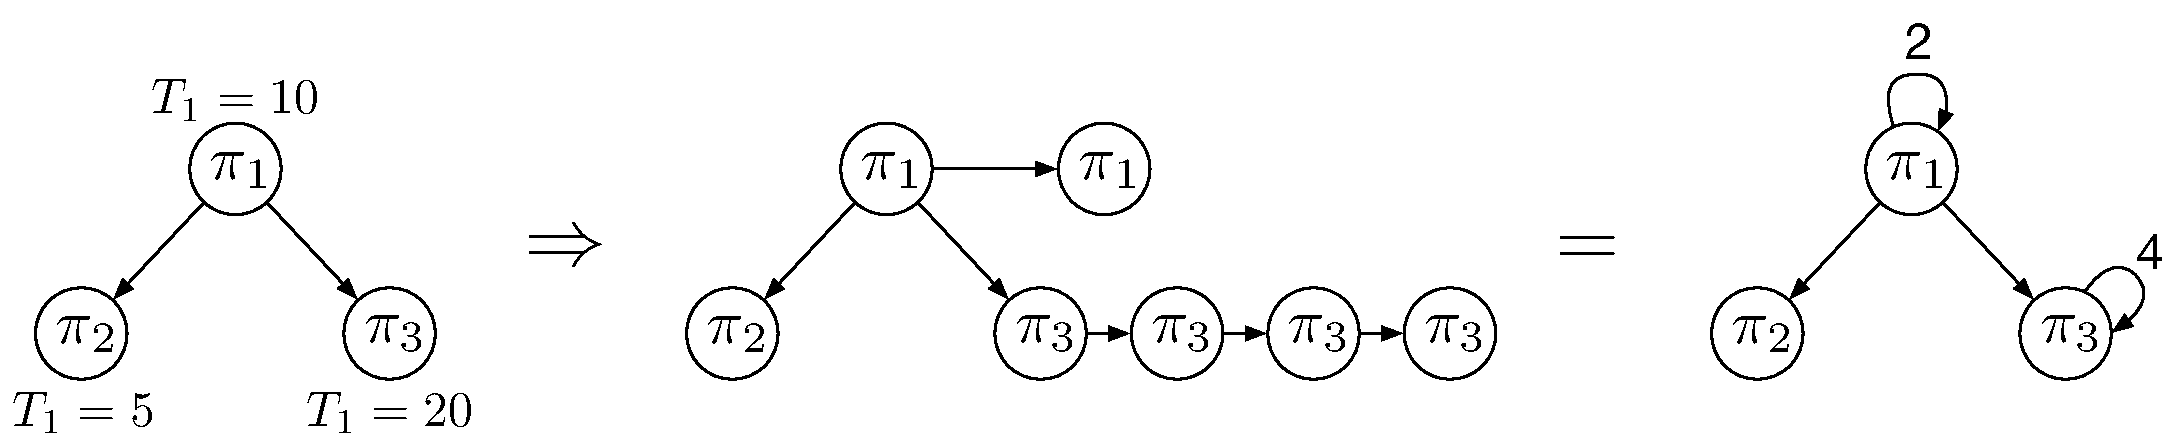
\includegraphics[width=1.0\textwidth]{Factorization}
\caption{Factorization example}
\label{fig:Factorization}
\end{figure}

\subsubsection{Partitions precedence constraints}
\par Given a schedule, it is called \emph{normal} if, for any two partition $\pi_i,\pi_j\in\Gamma$, $s_i<s_j$ implies that $\widetilde{d}_i\leq\widetilde{d}_j$ or $r_j>s_i$. Release times and deadlines are called \emph{consistent with the precedence relation} if $\pi_i\to\pi_j$ implies that $r_i+\delta t\leq r_j$ and $\widetilde{d}_i\leq\widetilde{d}_j-\delta t$, where $\delta t$ represent a small amount of time (basically the scheduling decision tick-time). The following lemma proves that the precedence constraints are not of essential relevance if there is only one processor.
\begin{lemma}\label{eq:precedenceLemma}
If the release times and deadlines are consistent with the precedence relation, then any normal one-processor schedule that satisfies the release times and deadlines must also obey the precedence relation. 
\end{lemma}
\begin{proof}
Consider a normal schedule, and suppose that $\pi_i\to\pi_j$ but $s_i>s_j$. By the consistency assumption we have $r_i<r_j$ and $\widetilde{d}_i<\widetilde{d}_j$. However, these, together with $r_j\leq s_j$, cause a violation of the assumption that the schedule is normal, a contradiction from which the result follows.
\end{proof}
This lemma ensures that release times and deadlines can be made consistent with the precedence relation if they are redefined by:
\begin{align}\label{eq:precedence}
r^{'}_{j} = & \max\big(\{r_j\}\cup\{r^{'}_i+\delta t:\pi_i\to\pi_j\} \big) \\
\widetilde{d}^{'}_j = & \min\big(\{\widetilde{d}_j\}\cup\{\widetilde{d}^{'}_i-\delta t:\pi_j\to\pi_i\} \big)
\end{align}
%\begin{align}
%r^{'}_{\alpha_j} = & \max\big(\{r_{\alpha_j}\}\cup\{r^{'}_{\alpha_i}+\delta t:\pi_{\alpha_i}\to\pi_{\alpha_j}\} \big) \\
%\widetilde{d}^{'}_{\alpha_j} = & \min\big(\{\widetilde{d}_{\alpha_j}\}\cup\{\widetilde{d}^{'}_{\alpha_i}-\delta t:\pi_{\alpha_j}\to\pi_{\alpha_i}\} \big)
%\end{align}
These changes do not alter the feasibility of any schedule. Furthermore, from lemma \ref{eq:precedenceLemma} follows that a precedence relation is essentially irrelevant when scheduling on one processor. 

\subsubsection{Bratley algorithm}
Scheduling partitions with precedence constraint (or adapted arrival times and due dates) is NP-hard in the strong sense, even for integer release times and deadlines \cite{LRKB77}. Only if all tasks have unit processing times, an optimization algorithm of polynomial time complexity is available. However, Bratley et al. \cite{bratleyScheduling} proposed a branch-and-bound algorithm which solves this class of problems. Their algorithm is shortly described below.
%Scheduling Computer and Manufacturing: Bratley et al. [BFR71] , page 74
\begin{figure}[htbp] 
\centering    
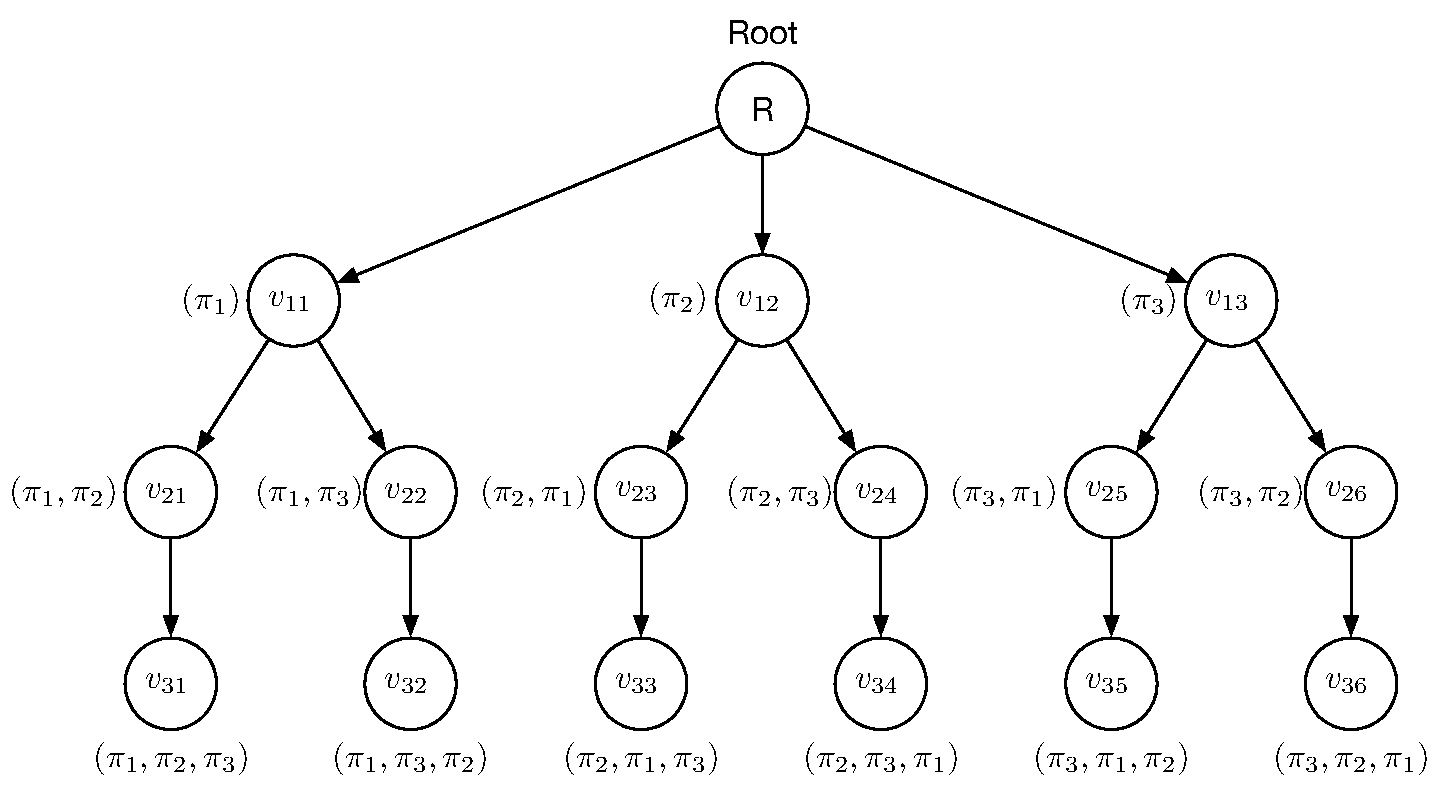
\includegraphics[width=1.0\textwidth]{Bratley}
\caption{Search tree example for Bratley et al. algorithm}
\label{fig:bratley}
\end{figure}
\paragraph{} All possible partition schedules are implicitly enumerated by a search tree as shown in Figure \ref{fig:bratley} (for three partitions). Each node $v_{ij}$ of the tree represents the assignment of $i-1$ partitions and a new unscheduled one to be in the $i$-th position of the schedule scheme, with $i = \{1,...,N\}$, $N=|\widetilde{\mathbb{P}}|$. On each level $i$, there are $N-i+1$ new nodes generated from each node of the preceding level. Hence, all the $N!$ possible schedule will be enumerated. To each node is associated the completion time of the corresponding partial schedule.
\par The order in which the nodes of the tree are examined is based on a \emph{backtracking
search strategy}. Moreover, the algorithm uses two criteria to bound the solution space.
\begin{enumerate}
\item Exceeding deadlines. Consider a node $v_{ij}$ of the tree where one of the $i$ partitions exceed its due date, it will certainly exceed its deadline if other partitions are scheduled after it. Therefore, the node with all the sub-tree may be excluded from further consideration.
\item Problem decomposition. Consider a node $v_{ij}$ where an unscheduled partition is assigned to $i$-th position of the schedule scheme. If the completion time of this partial schedule is less than or equal to the smallest release time among the yet unscheduled partitions, then the problem decomposes at level $i$, and there is need to backtrack beyond level $i$. This follows from the fact that the best schedule for the remaining $N-i$ partitions may not be started before the smallest of their release times.
\end{enumerate}
After enumerating all the possible $N!$ the best schedule according to an objective function can be selected. A common objective function is the makespan minimization.

%If the objective function is the makespan minimization, a sufficient but not necessary condition for optimality can be derived. Let define a \emph{block} as a group of partitions such that the first partition starts at its release time and all the following partitions to the end of the schedule are processed without idle times. Thus the length of a block is the sum of processing times of the partition within that block. If a block has the property that the release times of all the partitions within the block are greater than or equal to the release time of the first partition in the block (in that case we will say that \emph{"the block satisfies the release time property"}), then the schedule found for this block is clearly optimal. A block satisfying the release time property may be found by scanning the given schedule, starting from the last partition and attempting to find a group of tasks of the described property. Then, from the definition follow the lemma
%\begin{lemma}
%If a schedule for for a single-core, with starting time and due date, satisfies the release time property then it is one optimal solution for the makespan minimization.
%\end{lemma}

%********************************** % Section  **************************************
\section{Priority assignment}\label{sec:priorityassignment}
Priority assignment is required to allow the operating system scheduler to execute tasks according to the optimal schedule. 
\par Let assume that each thread has its affinity mask, meaning that it can execute only on the core specified by it and that the scheduler is priority-based FIFO queue. To enforce the non-preemptive behavior for the tasks inside a partition, threads on the same core must have \emph{strictly monotonically decreasing} priorities. Here to derive a correct assignment algorithm, an assumption on the implementation is required. Priorities alone cannot ensure mutual exclusion on communications memory locations. These shared memory regions are accessed only by communicating thread and them can be placed:
\begin{itemize}
\item On the same core: so priorities can ensure that the inputs are fulfilled, indeed the task with lower criticality will not execute before higher priority task.
\item On different core: so spinlocks can be used.
\end{itemize}
The use of spinlocks for inter-core synchronization is suggested because they avoid overhead from operating system process rescheduling or context switching. Moreover, spinlocks are efficient if tasks are likely to be blocked for only short periods, which is true to a certain degree that depends on the worst-case timing analysis. 

\paragraph{} A simple yet effective way to achieve this result is through a Linear Programming optimization problem:
\begin{equation}
\begin{cases}
\min \sum\rho_i \\ 
\rho_i - \rho_j \leq -1 \quad
\begin{matrix}
\text{for each consecutive task } \tau_i,\tau_j \text{ on the same core} \\
\text{for each communication edge } e_{ij} \text{ between cores}
\end{matrix} \\
\rho_{\min} \leq \rho_i \leq \rho_{\max}
\end{cases}
\end{equation}
where $\rho_i$ is the priority assigned to task $\tau_i\in\Gamma$. This class of problems can be solved in polynomial time \cite{polyLP}.

\paragraph{} Usually an operating system can only handle a finite set of priority values, for this reason the variable $\rho$ is bounded. However, if the schedule priority assignment does not use all the possible priority values, it is possible to create a gap below and above the partition to allow the execution of sporadic tasks. For example, this behavior can be easily implemented utilizing the background PikeOS partition \TP{0}. The result is depicted in figure \ref{fig:PriorityAssignment}.

\begin{figure}[htbp] 
\centering    
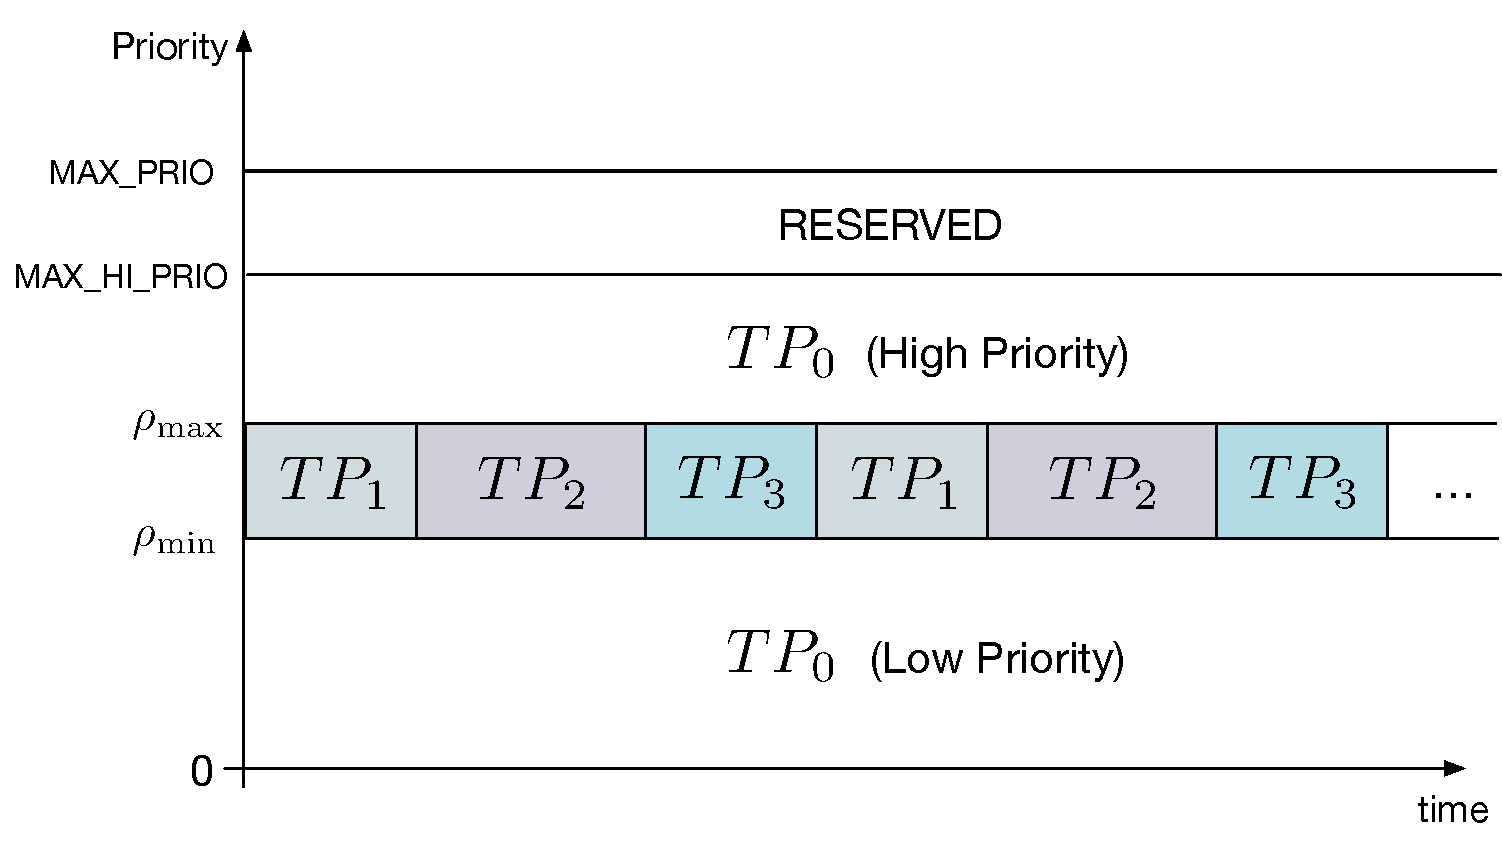
\includegraphics[width=1.0\textwidth]{PriorityAssignment}
\caption{Priority Assignment }
\label{fig:PriorityAssignment}
\end{figure}
